\section{Fehlerverhalten}
\label{Fehlervehalten}
Folgend ist beschrieben wie das System auf die injizierten Fehler reagiert und dadurch die Projektanforderungen an Zuverlässigkeit und Fehlertoleranz erfüllt.
\begin{figure}[H]
\centering
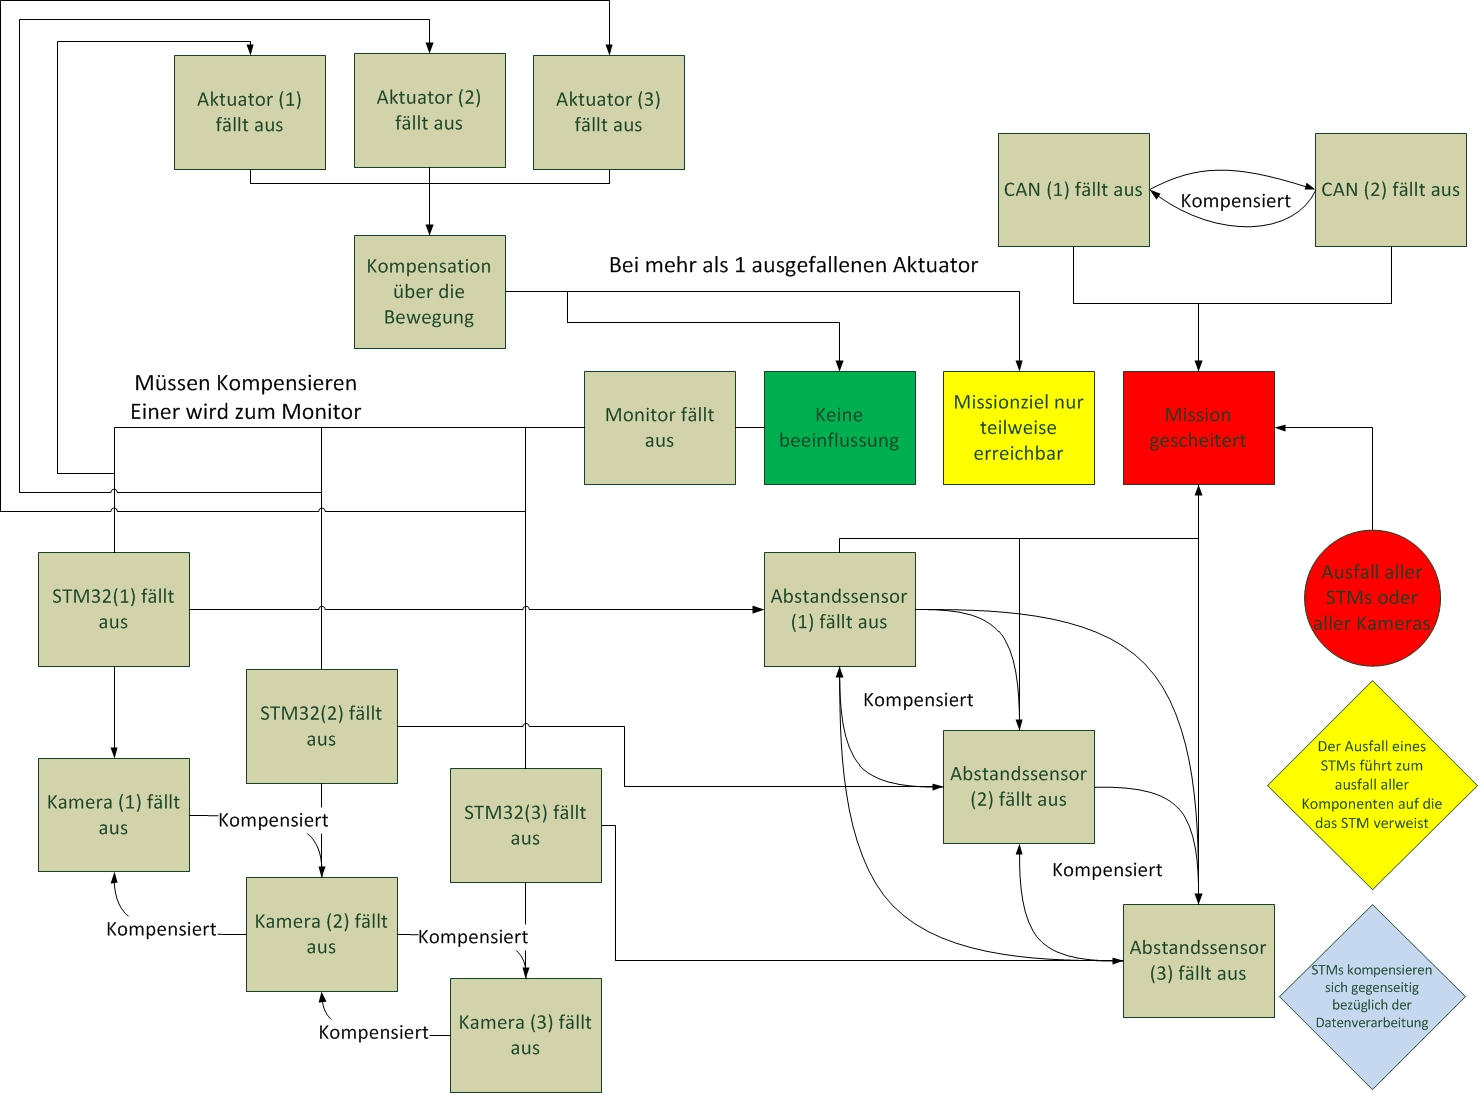
\includegraphics[width=\linewidth]{Bilder/FaTNet_fehlerverhalten}
\caption{Mögliche Fehlerfälle und entsprechende Kompensation}
\label{fig:fehlerverhalten}
\end{figure}

Bild \ref{fig:fehlerverhalten} veranschaulicht die verschiedenen Fehlerfälle, sowie die Möglichkeiten zu deren Kompensation grafisch.
Oben links in der Grafik wird gezeigt wie der Ausfall von Motoren am  Aktuator kompensiert wird.\\
Oben rechts sind die beiden CAN-Busse abgebildet, die ihren Ausfall wechselseitig kompensieren können.\\
Unten wird veranschaulicht, das System auf den Ausfall von STMs reagiert
Aus dem Systementwurf ergibt sich eine Ausfalltoleranz gegenüber bis zu zwei STMs, die Rechnungen bzw. die Steuerung wird dann  auf den/ die verbleibenden STM(s) ausgelagert um den Betrieb (unter Performanceeinbußen) fortzusetzen.\\
Da ein System nicht gegen jeden Komponentenausfall redundant sein kann, folgt eine Auflistung der konkreten Fehlerfälle mit denen das System umgehen kann. Alle Systemkomponenten, die nicht aufgelistet worden sind, wie z. B. die Antriebsmotoren und elektrischen Schaltungen und Leitungen, werden als \textit{Single Point of Failure} behandelt und sind nicht in der oberen Darstellung visualisiert. Das bedeutet, dass das System dann nicht in der Lage ist den Fehler zu finden und zu kompensieren.
Bild \ref{fig:fehlerverhalten} veranschaulicht die verschiedenen Fehlerfälle, sowie die Möglichkeiten zu deren Kompensation grafisch.


\paragraph{\textbf{Fehler 1: Ein STM fällt aus (siehe Abb. 8)}}$\;$\\
Das System verliert einen Aktuator, ein Abstandssensor sowie eine Kamera und abhängig vom ausgefallenen STM den Monitor.
Der fehlenden Aktuator reduziert den Freiheitsgrad des Manipulators, dadurch kann das Missionsziel bei mehr als einem ausgefallenen Aktuator nur noch teilweise erreicht werden. Der fehlende Freiheitsgrad kann durch das manövrieren des Demonstrators teilweise ausgeglichen werden, die ausgefallenen Abstandssensoren und Kameras wiederum schränken die Erfüllung des Missionsziels nicht ein, da diese redundant vorhanden sind.
Falls das ausgefallene STM in diesem Moment die Monitorfunktion übernahm, muss eines der verbliebenen STMs die Monitorfunktion übernehmen.

\begin{figure}[H]
\centering
  \begin{minipage}[b]{0.49\linewidth}
    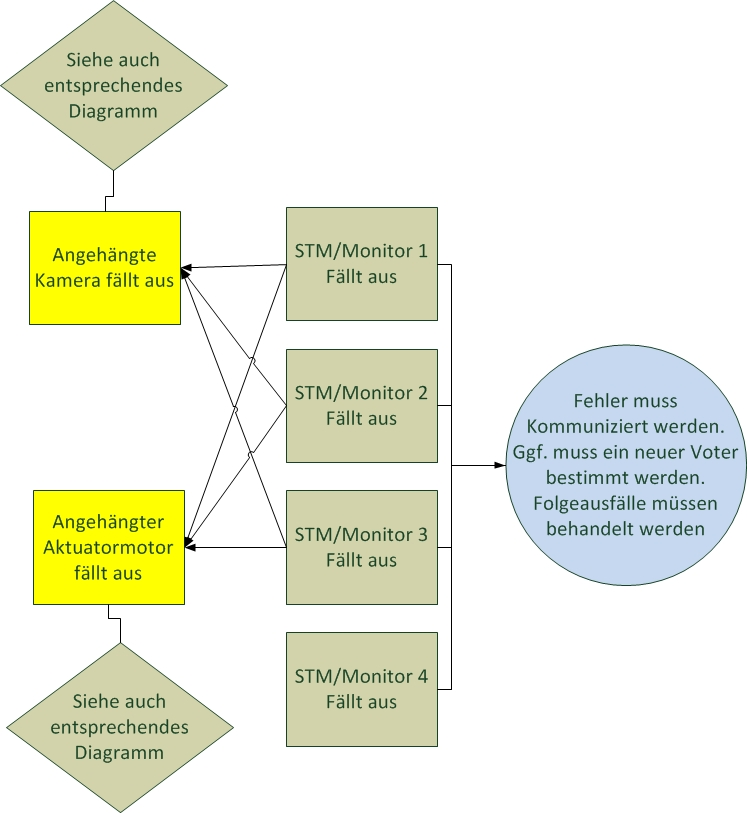
\includegraphics[width=\linewidth]{Bilder/FaTNet_stmredundanz} 
    \caption{Ausfall eines STM-Boards}
    \label{fig:stmredundanz}
  \end{minipage}
  \begin{minipage}[b]{0.49\linewidth}
    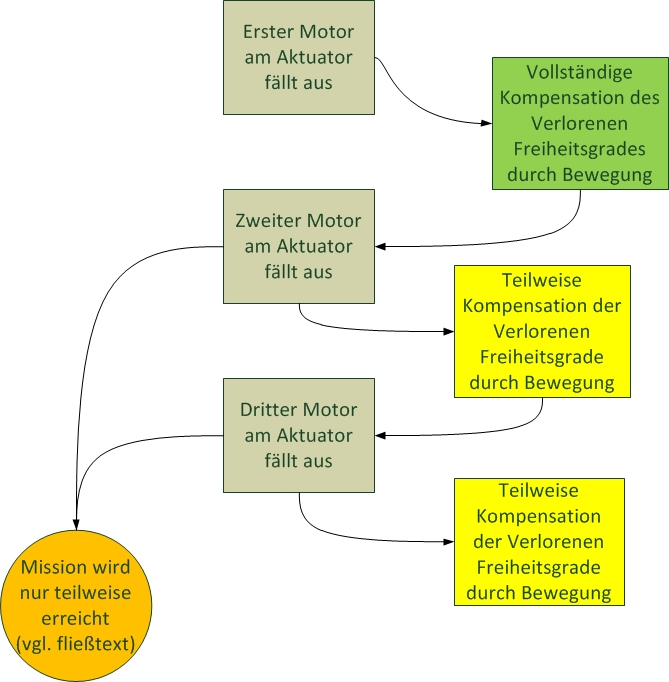
\includegraphics[width=\linewidth]{Bilder/FaTNet_aktuatorredundanz}  
    \caption{Ausfall eines  Aktuators}
    \label{fig:aktuatorredundanz}
  \end{minipage}
\end{figure}


\paragraph{\textbf{Fehler 2: Motor am Manipulator fällt aus (siehe Abb. 9)}}$\;$\\ 
Wie im Fehlerfall 1 kann das System den Verlust durch bewegen des Gesamtsystems teilweise kompensieren.
Wird ein ausgefallener Freiheitsgrad kompensiert ist der Manipulator immer noch in der Lage jede Raumposition anzufahren. Müssen zwei oder mehr ausgefallene Freiheitsgrade kompensiert werden kann es sein, dass der Manipulator nur eingeschränkte Raumpositionen anfahren kann. Dadurch kann das Missionsziel nur noch angenähert werden. Das System muss unter diesen Umständen das Ziel so gut es geht erreichen.

\paragraph{\textbf{Fehler 3: Monitor fällt aus (siehe Abb. 8)}}$\;$\\
Einer der anderen STMs übernimmt die Aufgabe des STM der vorher die Monitoraufgabe erfüllt hat, dadurch bleibt des Systems weiterhin voll funktionsfähig.
Die STMs sind intern durchnummeriert, das "ubriggebliebene STM mit der h"ochsten Nummer "ubernimmt die Funktion des Monitors.\\
Der Ablauf ist im Rahmen der STM-Redundanz erklärt.

\paragraph{\textbf{Fehler 4: Kamera fällt aus (siehe Abb. 10)}}$\;$\\
Es sind zwei Fehlerfälle möglich, zum Einen kann die Stromversorgung ausfallen, zum Anderen sendet die Kamera fehlerhafte Daten.
Falls die Stromversorgung für die Kamera ausfällt, übernehmen die redundanten Kameras die Funktion der ausgefallenen Kamera, dadurch bleibt das Missionsziel erreichbar.
Dieser Fehler wird dadurch erkannt das eine Kamera keine Daten mehr sendet.\\
Der zweite Fehlerfall, das senden falscher Daten, wird durch den Monitor kompensiert, d.h. der Monitor vergleicht die errechneten Daten und filtert die falschen Daten heraus.

\begin{figure}[H]
\centering
  \begin{minipage}[b]{0.49\linewidth}
    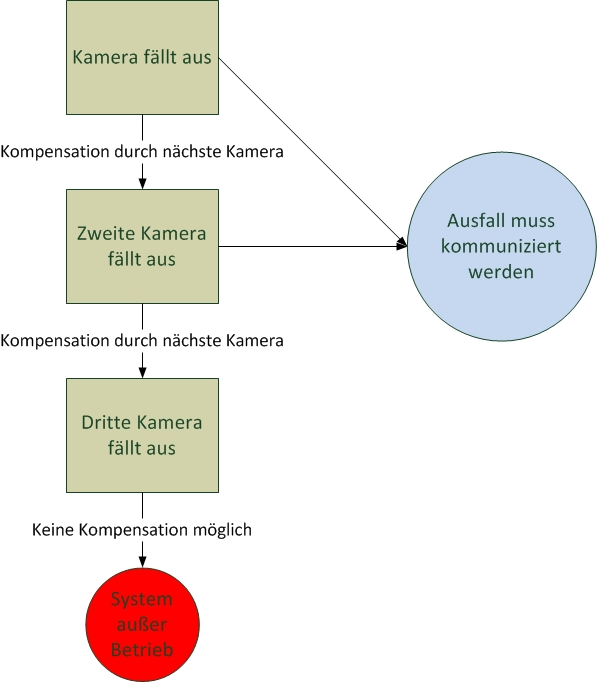
\includegraphics[width=\linewidth]{Bilder/FaTNet_kameraredundanz} 
    \caption{Ausfall einer Kamera}
    \label{fig:kameraredundanz}
  \end{minipage}
  \begin{minipage}[b]{0.49\linewidth}
    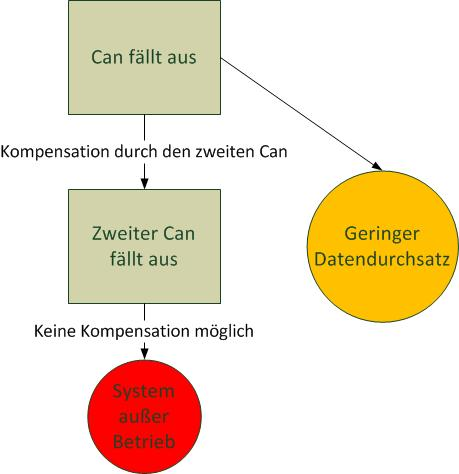
\includegraphics[width=\linewidth]{Bilder/FaTNet_canredundanz}  
    \caption{Ausfall eines CAN-Bus}
    \label{fig:canredundanz}
  \end{minipage}
\end{figure}

\paragraph{\textbf{Fehler 5: CAN-Bus fällt aus (siehe Abb. 11)}}$\;$\\
Der redundante CAN-Bus übernimmt die Aufgabe des ausgefallenen CAN-Bus, dadurch bleibt das System funktionsfähig.
Beim Ausfall des redundanten CAN-Bus ist keine weitere Kompensation mehr möglich und dementsprechend fällt das System aus.

\paragraph{\textbf{Fehler 6: Abstandssensor fällt aus (siehe Abb. 12)}}$\;$\\
Die redundanten Abstandssensoren übernehmen die Funktion der ausgefallenen Sensoren.
Der Ausfall eines Sensors wird dadurch ermittelt, dass dieser keine Daten mehr sendet.
\begin{figure}[H]
\centering
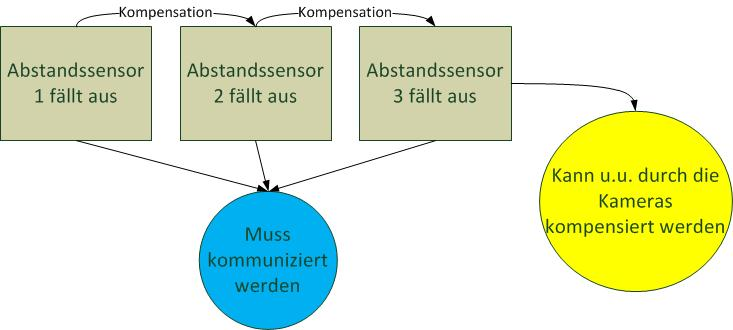
\includegraphics[width=0.7\linewidth]{Bilder/FaTNet_abstandssensoredundanz}
\caption{Ausfall eines Abstandssensors}
\label{fig:abstandssensorredundanz}
\end{figure}
